% -*- TeX:UTF-8 -*-
%%
%% KAIST 학위논문양식 LaTeX용 (ver 0.5) 예시
%%
%% @version 0.4
%% @author  채승병 Chae,Seungbyung (mailto:chess@kaist.ac.kr)
%% @date    2004. 11. 12.
%%
%% @requirement
%% teTeX, fpTeX, teTeX 등의 LaTeX2e 배포판
%% + 은광희 님의 HLaTeX 0.991 이상 버젼 또는 홍석호 님의 HPACK 1.0
%% : 설치에 대한 자세한 정보는 http://www.ktug.or.kr을 참조바랍니다.
%%
%% @note
%% 기존에 널리 쓰여오던 차재춘 님의 학위논문양식 클래스 파일의 형식을
%% 따르지 않고 전면적으로 다시 작성하였습니다. 논문 정보 입력부분에서
%% 과거 양식과 다른 부분이 많으니 아래 예시에 맞춰 바꿔주십시오.
%%
%%
%% @acknowledgement
%% 본 예시 논문은 물리학과 박사과정 김용현 님의 호의로 제공되었습니다.
%%
%% -------------------------------------------------------------------
%% @information
%% 이 예제 파일은 hangul-ucs를 사용합니다. UTF-8 입력 인코딩으로
%% 작성되었습니다. hlatex의 hfont는 이용하지 않습니다. --2006/02/11
%% 본 템플릿은 전산학부 김민혁 교수에의해서 버그 수정되었습니다. -- 2016/11/25

% @class kaist.cls
% @options [default: doctor, korean, final]
% - doctor: 박사과정 | master : 석사과정
% - korean: 한글논문 | english: 영문논문
% - final : 최종판   | draft  : 시험판
% - pdfdoc : 선택하지 않으면 북마크와 colorlink를 만들지 않습니다.


\documentclass[master,english,final]{kaist-ucs}


% If you want make pdf document (include bookmark, colorlink)
%\documentclass[doctor,english,final,pdfdoc]{kaist-ucs}

% kaist.cls 에서는 기본으로 dhucs, ifpdf, graphicx 패키지가 로드됩니다.
% 추가로 필요한 패키지가 있다면 주석을 풀고 적어넣으십시오,
%\usepackage{...}


% @command title 논문 제목(title of thesis)
% @options [default: (none)]
% - korean: 한글제목(korean title) | english: 영문제목(english title)
\title[korean] {양자 통신의 근원적 이론과 응용}
\title[english]{Theoretical Study on Quantum Communication with\linebreak Some Applications}

% @note 표지에 출력되는 제목을 강제로 줄바꿈하려면 \linebreak 을 삽입.
%       \\ 나 \newline 등을 사용하면 안됩니다. (아래는 예시)
%
%\title[korean]{탄소 나노튜브의 물리적 특성에 대한\linebreak 이론 연구}
%\title[english]{Theoretical study on physical properties of\linebreak
%                carbon nanotubes}
%
% If you want to begin a new line in cover, use \linebreak .
% See examples above.
%


% @command author 저자 이름
% @param   family_name, given_name 성, 이름을 구분해서 입력
% @options [default: (none)]
% - korean: 한글이름 | chinese: 한문이름 | english: 영문이름
% 한문 이름이 없다면 빈 칸으로 두셔도 됩니다.
%
%
% If you are a foreigner , write your name in korean or your korean name.
% If you can't write native character, you can make the chinese blank empty 
% Write as follow
% \author[korean]{family name in korean}{given name in korean}
% \author[chinese]{family name in your native language}{given name in your native language}
% \author[english]{family name in english}{given name in english}
%
\author[korean]{박}{상 우}
\author[korean2]{박}{상우}    %이름을 붙여 써 주시기 바랍니다.
\author[chinese]{朴}{相 禹}
\author[english]{Park}{Sangwoo}

% @command advisor 지도교수 이름 (복수가능)
% @usage   \advisor[options]{...한글이름...}{...영문이름...}{signed|nosign}
% @options [default: major]
% - major: 주 지도교수  | coopr: 공동 지도교수
\advisor[major]{송 익 호}{Iickho Song}{signed}
\advisor[major2]{송익호}{Iickho Song}{signed}    %한글 성과 한글 이름을 모두 붙여 써 주시기 바랍니다.
\advisorinfo{Professor of Electrical Engineering} %제출승인서에 들어가는 교수님 정보, advisor's information 
%\advisor[coopr]{홍 길 동}{Gil-Dong Hong}{nosign}
%\advisor[coopr2]{홍길동}{Gil-Dong Hong}{nosign}    %한글 성과 한글 이름을 모두 붙여 써 주시기 바랍니다.
%
% 지도교수 한글이름은 입력하지 않아도 됩니다.
% You may not input advisor's korean name
% like this \advisor[major]{}{Chang, Kee Joo}{signed}
%


% @command department {학과이름}{학위종류} - 아래 규칙에 따라 코드를 입력
% @command department {department code}{degree field}
%
% department code
% 2. 석박사학위논문 작성 및 제출요령 4쪽 ~ 5쪽 참고
% 또는 kaist-ucs.cls 의 % @command department 참고

% science: 이학 | engineering: 공학 | business : 경영학
% 박사논문의 경우는 학위종류를 입력하지 않아도 됩니다.
% If you write Ph.D. dissertation, you cannot input degree field.
% The third parameter : a | b | c
% a: 소속된 학과만 쓰는 옵션 (학과에만 소속되어 있는 경우에는 무조건 a를 선택해야 함)
% b: 학과 아래의, 프로그램이나 학제전공에 소속되어 있을 경우에 학과와 프로그램을 함께 쓰는 옵션
% c: 학과 아래의, 프로그램이나 학제전공에 소속되어 있을 경우에 학과를 쓰지 않고 프로그램이나 학제전공의 이름만 쓰는 옵션 
% 
% a: it represents only the name of department. (if you aren't in the program under the department, must choose a)
% b: it represents the names of department and the program that is under the department (consider this when you are in the program not only department)
% c: it represents only the name of program that is under the department (consider this when you are in the program not only department)
\department{PH}{engineering}{a}

% @command referee 심사위원 (석사과정 3인, 박사과정 5인)
\referee[1]{송 익 호}
\referee[2]{안 진 현}
\referee[3]{정 태 성}
\referee[4]{가 동 호}
\referee[5]{박 태 현}
% \referee[5] {Barack Obama}
% Of course english name is available

% @command approvaldate 지도교수논문승인일
% @param   year,month,day 연,월,일 순으로 입력
\approvaldate{2020}{12}{5}

% @command refereedate 심사위원논문심사일
% @param   year,month,day 연,월,일 순으로 입력
\refereedate{2020}{12}{5}

% @command gradyear 졸업년도
\gradyear{2020}

% 본문 시작
\begin{document}

    % 앞표지, 속표지, 학위논문 제출승인서, 학위논문 심사완료 검인서는
    % 클래스 옵션을 final로 지정해주면 자동으로 생성되며,
    % 반대로 옵션을 draft로 지정해주면 생성되지 않습니다.

    % 논문 서지, 초록, 핵심 낱말, 영문 초록, 영어 핵심 낱말 (Information of thesis, abstract in korean, keywords in korean, abstract in english, keywords in english)
   \thesisinfo
   %% Letters of abstract in korean must be less than 500 and words of abstract in english must be less than 300.
   %% Number of keywords must be less than 6.
   %% Don't write english letters in the abstract in korean.
    \begin{summary}      
    이 논문에서는 부 쓰는이가 여러 안테나를 쓰는 협력 인지 무선통신망을 다루었다. 안테나 개수는 이제까지의 방법과 같도록 유지하면서 부 쓰는이가 다다를 수 있는 전송률을 높이는 방안을 제시하였다. 좀 더 자세히 말하면, 동시 송수신 안테나를 써서 부 쓰는이끼리 전 이중으로 신호를 주고받을 수 있게 하여 부 쓰는이가 다다를 수 있는 전송률을 높이는 방안을 제시하고 그 성능을 살펴보았다. 제안한 협력 인지 무선통신망이 나타내는 다다를 수 있는 전송률이 이제까지의 다른 협력 인지 무선통신망에서 얻을 수 있는 것과 견주어 꽤 높음을 해석적인 방법과 계산적인 방법으로 보였다.

    \end{summary}
   
    \begin{Korkeyword}
    인지 무선 통신, 협력 통신, 중계, 전 이중, 동시 송수신
    \end{Korkeyword}


    \begin{abstract}
    We address cooperative cognitive radio networks (CCRNs) with secondary users (SUs) exploiting multiple antennas. In order to expand the achievable rate region by enabling full-duplex communication between SUs, we adopt simultaneous transmitting and receiving antennas for the SUs. The link capacities of the proposed framework are analyzed theoretically. It is shown through numerical analysis that the proposed framework can provide a considerable performance gain over the conventional CCRN framework.
    \end{abstract} 
     
    \begin{Engkeyword}
    Cognitive radio, cooperation communication, relay, full-duplex, simultaneous transmission and reception
    \end{Engkeyword}
   

    \addtocounter{pagemarker}{1}                 % 백색별지분을 고려
    \newpage 
  


    % 목차 (Table of Contents) 생성
    \tableofcontents

    % 표목차 (List of Tables) 생성
    \listoftables

    % 그림목차 (List of Figures) 생성
    \listoffigures

    % 위의 세 종류의 목차는 한꺼번에 다음 명령으로 생성할 수도 있습니다.
    %\makecontents

%% 이하의 본문은 LaTeX 표준 클래스 report 양식에 준하여 작성하시면 됩니다.
%% 하지만 part는 사용하지 못하도록 제거하였으므로, chapter가 문서 내의
%% 최상위 분류 단위가 됩니다.
%% You cannot use 'part'

\chapter{Introduction}
\noindent
Cognitive radio (CR), a key technology of resource-efficient wireless communications, can be employed to solve the problem of frequency resource shortage. However, due to the uncertainty of the secondary users' (SUs') usage of frequency band, the original CR has failed to gain sufficient interests. Recently, a new paradigm termed cooperative cognitive radio networks (CCRNs) has been proposed \cite{FD1}-\cite{ML1}...

There ...

\chapter[Related Works and Contributions of this Dissertation]{Related Works and \\ Contributions of this Dissertation}

\section{Quantum Communication}

There have been extensive studies on cognitive radio in recent years. To enhance the performance gain of original cognitive radio networks (CRNs), leveraging cooperative diversity has attracted a lot of attention \cite{SOCA1}...

\subsection{Examples}


\section{Applications of Quantum Communication}

Despite its potential to improve the throughput, spatial domain diversity was not fully considered in the studies of original CCRNs. Utilizing the spatial domain for the communications, the concept of MIMO has been adopted in many cases to increase the wireless capacity \cite{EF1,FD2}...


\chapter{Proposed Architecture and Its Application}

\section{Proposed Architecture}

Let us consider an MIMO-CCRN with one PL and one SL. Each PU has one legacy antenna and each SU has two STAR antennas. The duration of one communication time frame is divided into two phases \cite{RVP2,ML2} ...
%%
%% 표 삽입 예시
%% Example. how to insert table
%%
\begin{table}[t]
\caption[Enter the caption title here]{Energy stability $E$ (eV) per molecule of all meta-stable
isomer states of C$_{60}$ opening process for forming the (5,5) cap.
In the SW-I and SW-II, both ferromagnetic (Ferro) and paramagnetic (Para)
spin configurations are obtained, whereas only non-magnetic configuration
is obtained in the BF, SW-III, and CAP(5,5).
$M$ is total magnetization $n_{\rm up}$-$n_{\rm down}$ in unit of $\mu_B$, where
$n_{\rm up(down)}$ is the number of up (down) spins.
}
\label{mag-tab1}
\begin{center}
\begin{tabular} {ccccccccccc}
\hline\hline
& & BF &\multicolumn{2}{c}{SW-I}&&\multicolumn{2}{c}{SW-II}&SW-III&CAP&\\
\cline{4-5} \cline{7-8}
&               &   &  Para & Ferro &&   Para &  Ferro &      &      &\\
\hline
& $E$ (eV)      & 0 & 7.796 & 7.832 && 10.418 & 10.408 & 11.5 & 13.2 &\\
& $M$ ($\mu_B$) & 0 &     0 &  1.94 &&      0 &   2.06 &    0 &    0 &\\
\hline\hline
\end{tabular}
\end{center}
\end{table}

%%
%% 그림 삽입 예시
%% Example. how to insert graph
%%
%% Note. 가급적 \includegraphics 명령을 사용하십시오.
%% Recommen : Use \includegraphics to insert graph.
%%
\begin{figure}[t]
    \centerline{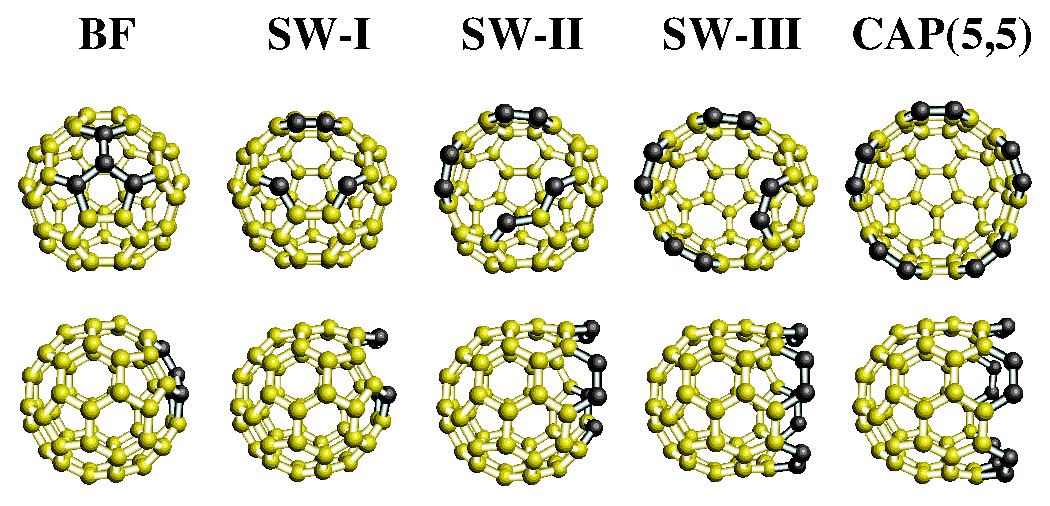
\includegraphics[width=12.5cm]{sample-fig1}}
    \caption[Enter the caption title here]{ Ball-and-stick models of meta-stable isomers in
        cage opening process from a C$_{60}$ buckminsterfullerene
        to a (5,5) capsule. We name them BF and CAP(5,5).
        Depending on the number of the Stone-Wales (SW) transformation,
        we call the intermediate isomers with SW-I, SW-II, and SW-III.
        Highlighted atoms are undercoordinated except BF.
    } \label{mag-fig1}
\end{figure}

\section{Application}

The achievable rates can be calculated by finding the statistics of the five signals transmitted that maximize the mutual information between $s_{t,XY}$ and $y_{t,XY}$ for $(X,Y)=(T,C), (C,N)$, and $(N,C)$ when $t=1$, and $(X,Y)=(C,R), (C,N)$, and $(N,C)$ when $t=2$ \cite{SOCA2,EF2}...


\chapter{Concluding Remark}

We have proposed a novel FD MIMO-CCRN framework providing a reasonable performance improvement compared with the conventional MIMO-CCRN framework...
%%
%% 참고문헌 시작
%% bibliography
%% It can be changed but should include sufficient information.
\begin{thebibliography}{00}

\bibitem{FD1} 박상우, \underline{동시 송수신 안테나를 두 개 쓰는 협력 인지 무선통신망에 알맞은 전 이중 통신}, 한국과학기술원 석사 학위 논문, 2016.

\bibitem{RVP1} 송익호, 박철훈, 김광순, 박소령, \underline{확률변수와 확률과정}, 자유아카데미, 2014.

\bibitem{ML1} 송익호, 안태훈, 민황기, \underline{인지 무선에서의 광대역 주파수 검출 방법 및 장치}, 특허등록번호 10-1494966, 2015년 2월 12일.

\bibitem{SOCA1} 호우위시, 이원주, 이승원, 안태훈, 이선영, 민황기, 송익호, “선형 판별 분석에서 부류안 분산 행렬의 영 공간 재공식화,” \underline{한국통신학회 2012년도 추계종합학술발표회}, 대한민국 고려대학교, 242-243쪽, 2012년 11월.

\bibitem{EF1} 민황기, 안태훈, 이승원, 이성로, 송익호, “비간섭 전력 부하 감시용 고차 적률 특징을 갖는 전력 신호 인식,” \underline{한국통신학회논문지}, 제39C권, 제7호, 608-614쪽, 2014년 7월.



\bibitem{FD2} S. Park, \textit{Full-Duplex Communication for Cooperative Cognitive Radio Networks with Two Simultaneous Transmit and Receive Antennas}, Master Thesis, Korea Adv. Inst. Science, Techn., Daejeon, Republic of Korea, 2016.

\bibitem{RVP2}  I. Song, J. Bae, and S. Y. Kim, \textit{Advanced Theory of Signal Detection: Weak Signal Detection in Generalized Observations}, Springer-Verlag, 2002.

\bibitem{ML2} I. Song, T. An, and J. Oh, \textit{Near ML decoding method based on metric-first search and branch length threshold,} registration no. US 8018828 B2, Sep. 13, 2011, USA. 

\bibitem{SOCA2} H.-K. Min, T. An, S. Lee, and I. Song, “Non-intrusive appliance load monitoring with feature extraction from higher order moments,” in \textit{Proc. 6th IEEE Int. Conf. Service Oriented Computing, Appl.,} Kauai, HI, USA, pp. 348-350, Dec. 2013.

\bibitem{EF2} I. Song and S. Lee, “Explicit formulae for product moments of multivariate Gaussian random variables,” \textit{Statistics, Probability Lett.,} vol. 100, pp. 27-34, May 2015.


\end{thebibliography}



%%
%% 감사의 글 시작
%% Acknowledgement
%%
% @command acknowledgement 감사의글
% @options [1 | 2 | 3 |4 ]
% - 1 : 본문과 감사의 글이 둘 다 한글일 때  | 2 : 본문은 한글인데 감사의 글이 영어일 때 | 3 :  본문과 감사의 글이 둘 다 영어일 때  | 4 : 본문은 영어인데 감사의 글이 % 한글일 때 
%% It is optional.

\acknowledgment[4]
    언제나 저를 바른 길로 이끌어 주시는 송익호 교수님께 큰 고마움을 느낍니다.
    끝으로 오늘의 제가 있을 수 있도록 사랑으로 키워 주신 가족들에게 감사드립니다.
    저의 이 작은 결실이 그분들께 조금이나마 보답이 되기를 바랍니다.

%%
%% 약력 시작
%% Curriculum Vitae
%%
% @command curriculumvitae 이력서
% @options [1 | 2 | 3 |4 ]
% - 1 : 본문과 약력이 둘 다 한글일 때  | 2 : 본문은 한글인데 약력이 영어일 때 | 3 :  본문과 약력이 둘 다 영어일 때  | 4 : 본문은 영어인데 약력이 한글일 때 
%% It is optional and you can change form of this in the class file if you want.
\curriculumvitae[4]

    % @environment personaldata 개인정보
    % @command     name         이름
    %              dateofbirth  생년월일
    %              birthplace   출생지
    %              domicile     본적지
    %              address      주소지
    %              email        E-mail 주소
    % - 위 6개의 기본 필드 중에 이력서에 적고 싶은 정보를 입력
    % input data only you want
    \begin{personaldata}
        \name       {박 상 우}
        \dateofbirth{19xx}{xx}{xx}
        \birthplace {...}
        \address    {...}
    \end{personaldata}

    % @environment education 학력
    % @options [default: (none)] - 수학기간을 입력
    \begin{education}
        \item[2008. 3.\ --\ 2010. 2.] 고등학교 (2년 수료)
        \item[2010. 2.\ --\ 2014. 2.] 한국과학기술원 물리학과 (학사)
        \item[2014. 3.\ --\ 2016. 2.] 한국과학기술원 전기및전자공학부 (석사)
    \end{education}

    % @environment career 경력
    % @options [default: (none)] - 해당기간을 입력
    \begin{career}
        \item[2015. 3.\ --\ 2016. 2.] 한국과학기술원 전기및전자공학부 조교
    \end{career}

    % @environment activity 학회활동
    % @options [default: (none)] - 활동내용을 입력
%%    \begin{activity}
%%        \item J. Choi, \textbf{Yong-Hyun Kim}, K.J. Chang, and D. Tomanek,
%%             \textit{Occurrence of itinerant ferromagnetism in C/BN superlattice
%%             nanotubes}, 5th Asian Workshop on First-Principles Electronic
%%             Structure Calculations, Seoul (Korea), October., 2002.
%%    \end{activity}

    % @environment publication 연구업적
    % @options [default: (none)] - 출판내용을 입력
    \begin{publication}
        %\item \textbf{Yong-Hyun Kim}, J. Choi, K.J. Chang, and D. Tomanek,
        %     \textit{Magnetic instability in partly opened C$_{60}$ isomers},
        %     in preparation.
        \item H.-K. Min, Y. Hou, {\bf S. Park}, and I. Song,
``A computationally efficient scheme for feature extraction with kernel discriminant analysis,"
\textit{Patt. Recogn.}, vol.~50, no.~2, pp.~45-55, Feb. 2016 (to be published).
    \end{publication}

  \label{paperlastpagelabel}     % <-- 추가 부분: 마지막 페이지 위치 지정	
%% 본문 끝
\end{document}
